\documentclass[../mit-general-chemistry.tex]{subfiles}
\begin{document}



\chapter{Thermodynamics in biological systems}

Let's look at thermodynamics in biological systems.


\section{ATP-coupled reactions}


Many reactions within the living cell are non-spontaneous in
themselves. 



Many biological reactions are non-spontaneous, so to ``drive'' the
reactions the cell uses {\em ATP hydrolyzis}. The hydrolysis of ATP
can be coupled to a non-spontaneous process to drive the reaction
forward.

Consider a reaction

\begin{center}
  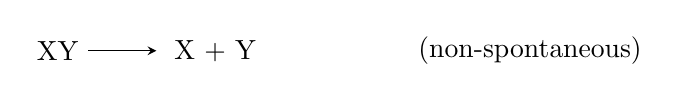
\begin{tikzpicture}[font=\normalfont]
    \node at (-1, 0) (r) {\ce{XY}};
    \node at (1, 0) (p) {\ce{X + Y}};
    \draw[->,>=stealth,shorten >=3pt] (r) -- (p);
    \node at (5, 0) (p) {(non-spontaneous)};
  \end{tikzpicture}
\end{center}

for some elemtns \ce{X} and \ce{Y}, and assume that the reaction is
non-spontaneous (endergonic) in the forward direction. By coupling the reaction to
the hydrolysis of \ce{ATP}, the total changr in free energy of the the
coupled reaction is the sum of the free energy of the individual
reactions.

So the body couples the non-spontaneous reaction with the spontaneous
ATP hydrolysis reaction.




\subsection{ATP}


\ceeqstar{ATP + H2O -> ADP + PO4^2- + H3O+}

The {\em ATP cycle} is an ever continuing process where the cell
stores energy from aerobic respiration and fermentation in one step
and releases that energy in the next. It is the link between our
intake of food and putting that energy to work. Every 24 hours, it has
been said, the body uses it's weight of ATP in different reactions
throughout the body. Meanwhile it only contains around \SI{100}{\gram}
of actual molecules. The figures are, of course, supposed to be taken
lightly but points to the incredible fact. This is possible thanks to
constant recycling and ``recharging'' of ATP/ADP molecules, who are in
themselves not actually consumed in the reaction, but merely used as a
``battery''. The usage and recharging of ATP occurs in a process,
called {\em the ATP cycle}.


\begin{figure}[h]
  \begin{margincap}
    \begin{center}
      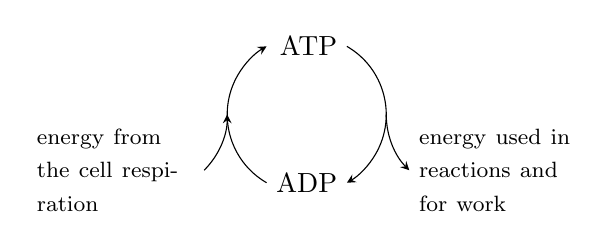
\begin{tikzpicture}[font=\normalfont]
        \def\radius{1cm}
        \draw[->,>=stealth] (0, 0cm)
        arc[start angle=60, end angle=-60, radius=\radius]
        node[at start, left] (atp) {ATP}
        node[at end, left] (adp) {ADP}
        node[midway] (mw1) {};
        \draw[->,>=stealth] (adp.west)
        arc[radius=\radius, start angle=240, end angle=120]
        node[midway] (mw2) {};
        \draw[->,>=stealth] (mw1)
        arc[start angle=180, end angle=225, radius=\radius]
        node[at end,right, text width=2cm] {\footnotesize energy used in reactions and
        for work};
        \draw[<-,>=stealth] (mw2)
        arc[start angle=0, end angle=-45, radius=\radius]
        node[at end,left, text width=2cm] {\footnotesize energy from the cell respiration};
      \end{tikzpicture}
    \end{center}
    \caption{The ATP cycle links the cell respiration to the energy
      requiring processes of the body.}
  \end{margincap}
\end{figure}







\subsection{Coupling reactions}


By coupling exorgonic reactions to endorgonic reactions, the body can
control and drive the endorgonic reactions. These reactions are ofte
enzymatic, they are enabled by the presence and participation of
enzymes.

\begin{center}
  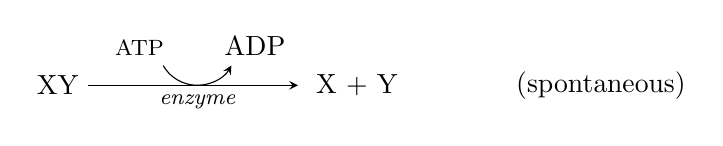
\begin{tikzpicture}[font=\normalfont]
    \node at (-1.9, 0) (r) {\ce{XY}};
    \node at (1.9, 0) (p) {\ce{X + Y}};
    \draw[->,>=stealth,shorten >=3pt] (r) -- (p)
    node[midway] (midarrow){}
    node[midway,below] {\em\footnotesize enzyme};
    
    \draw[->,>=stealth] (midarrow) arc[radius=.5cm, start angle=270, end angle=330]
    node [at end, above,xshift=3mm] (aboveU) {ADP};

    \draw (midarrow) arc[radius=.5cm, start angle=270, end angle=210]
    node [at end, above,xshift=-3mm] {\footnotesize ATP};

    \node at (5, 0) (p) {(spontaneous)};
  \end{tikzpicture}
\end{center}

%\schemestart
% A
% \arrow{-y>[a][b][enzyme]}
% B
%\schemestop



\subsubsection{Calculate the free energy of ATP hydrolysis}

To calculate the free energy of the hydrolysis of ATP we remember from
earlier calculations that $\enthalpy^0 = -24~\kjpm$. We can also find
that $\dS^0 = \SI{22}{\joule\per\kelvin\per\mol}$. A normal
temperature of a human body might be \SI{310}{\kelvin}.

\begin{align*}
  \gibbs^0 &= \enthalpy^0 - T \cdot \dS^0 =\\
  &=  -24~\kjpm - \SI{310}{\kelvin} \cdot \SI{0.022}{\kilo\joule\per\kelvin\per\mol} =\\
  &= \SI{-31}{\kilo\joule\per\mol} \\
\end{align*}
We get a negative \gibbs which is what we expected. This means that
this reaction has excess energy to use to drive non-spontaneous
reactions.

Besides the energy transfer ATP is used in phosphorylation of
molecules for different effects, such as turning functions of proteins
on and off.




\subsubsection{Glucose phosphorylation}


Glucose is an important source of energy for the living cell. It is
transported through the cell membrane by active transport, facilitated
by families of membrane transport proteins, {\em glucose
  transporters}.

Inside the cell, hexokinase enzymes mediate the phosphorylation of the
glucose molecule. This adds a phosphate group from an ATP molecule on
the sixth carbon atom of the glucose. This prevents the glucose
molecule from leaving the cell which increases the level of glucose
inside the cell against it's concentration gradient. The reaction is
non-spontaneous and occur coupled to ATP hydrolysis.


Let's look at a reaction that is coupled with ATP hydrolysis. Glucose
is an non-polar molecule. This means it can move freely across the
(non-polar) lipid cell membrane. Through phosphorylation of the glucose
molecule a phosphate group is added on the sixth carbon of the
molecule. This makes the glucose (now glucose-6-P) molecule polar,
because of the electric charge of \ce{HPO3-}. As this occurs inside the cell,
the glucose molecule can no longer leave the cell.

\begin{hfigure}
  \vspace{1em}
  \begin{center}
    \begin{tikzpicture}
      \coordinate (z) (0, 0);
      \node[left=1.5cm of z] (a) {glucose \ce{C6H12O6}};
      \node[right=1.5cm of z] (b) {glucose-6-phosphate \ce{C6H13O9P}};
      \node[above=of a] (am) {\chemfig{[:-120]*6((-[:90]-[:60]OH)-(-[:150]OH)-(-[:210]OH)-(-[:270]OH)-(-[:330]OH)-O-)}};
      \node[above=of b] (bm) {\chemfig{[:-120]*6((-[:90]-[:60]O(-[:90]P(=[:90]O)(-[:0]OH)(-[:180]HO)))-(-[:150]OH)-(-[:210]OH)-(-[:270]OH)-(-[:330]OH)-O-)}};
      \draw[->,shorten <=.5cm,shorten >=.5cm] ($(z) + (-1.5, 2.5)$) -- ($(z) + (1.5, 2.5)$)
      node[midway] (arrow){}
      node[midway,below] {\em hexokinase};
      \draw[->] (arrow) arc[start angle=270, end angle=315, radius=1cm]
      node[at end, above]{\footnotesize ADP};;
      \draw (arrow) arc[start angle=270, end angle=225, radius=1cm]
      node[at end, above]{\footnotesize ATP};
    \end{tikzpicture}
  \end{center}
  \caption{
    Glucose phosphorylation is a mechanism within the cell to
    prevent glucose to leave the cell, once it has entered.  Glucose
    is a non-polar molecule in itself. This enables glucose
    molecules to freely pass through the cell membranes. The
    phosphate group makes the molecule polar and this prevents the
    molecule from passing through the lipid membrane of the
    cell. The reaction is non-spontaneous and have but occur coupled
    to ATP hydrolysis.
  }
\end{hfigure}




This reaction requires energy, $\gibbs =
\SI{17}{\kilo\joule\per\mol}$. To have this reaction occur it is
coupled with ATP hydrolysis in the cell and if we calculate the free
energy for the coupled reaction we get
\begin{align*}
  \gibbs_{\text{total}} &=
  \gibbs_{\text{phosphorylation}} + \gibbs_{\text{hydrolysis}} =\\ 
  &= \SI{17}{\kilo\joule\per\mol} - \SI{31}{\kilo\joule\per\mol} =\\
  &= \SI{-14}{\kilo\joule\per\mol} \\
\end{align*}
which is a spontaneous reaction.

To spend ATP to control unfavoured reactions is very common in living
cells. This is why ATP is called the energy currency of cell
biology. Some reactions require one mole equivalent of ATP to occur,
other require more.







\section{Hydrogen bonds}



Hydrogen bonds are {\em inter-molecular} bonds. A hydrogen bond is
formed between a hydrogen atom that is partially positive (due to it's
containing compound) and a partially negative {\em hydrogen bond donor
  atom} with a lone pair of electrons.

\vspace{2em}
\hspace*{\fill}
$\chemfig{
    X-\chemabove{H}{\scriptsize\delta +}
}$
\hfill
$\chemfig{
    \chemabove{\lewis{4:,Y}}{\scriptsize\delta -}-
}$
\hspace*{\fill}

\vspace{.5em}
\hspace*{\fill}
$\chemfig{
    X-\chemabove{H}{\scriptsize\delta +}-[,,,,dash bond]\chemabove{\lewis{4:,Y}}{\scriptsize\delta -}-
}$
\hspace*{\fill}

Hydrogen bonds are commonly drawn with a dashed line to distinguish
them from covalent bonds that is drawn with a solid, straight line.

The atom that the hydrogen atom is bound to (the \ce{X} in the
illustration above) and the hydrogen bond donor (the \ce{Y} in the
illustration above) must be of an element with really high
electronegativity, such as nitrogen, oxygen or fluoride. This make
sense as the atoms need to be fairly small, be highly electronegative
and have a lone pair of electrons.

Water molecules form hydrogen bonds among each other. We draw two
water molecules.

\begin{center}
  \chemfig[remember picture]{
    H
    -[:38]
    \lewis{1:3:,O}
    -[:-38]@{h1}H
    -[:-38,,,,dash bond]
    @{o1}\lewis{3:5:,O}
    (-[:-38]H)
    (-[:67]H)
  }
  \chemmove{
    \node[yshift=-.2mm,xshift=-3mm] at (o1) {\color{red}$\scriptsize\delta^-$};
    \node[yshift=-2mm,xshift=-2mm] at (h1) {\color{red}$\scriptsize\delta^+$};
  }
\end{center}

The hydrogen bond is strongest and most stable when the atoms are all
lined up in a straight line. The hydrogen bonds are weaker than
covalent bonds and are, accordingly, longer as well. The mean enthalpy
for a hydrogen bond tend to be five percent of that of the
corresponding covalent bonds (as seen in
Table~\ref{tbl:hydrogenbondenthalpy}) so it is a weak bond, compared
to covalent bonds. The hydrogen bond is, however, the strongest
among the inter-molecular bonds.

\begin{htable}
  \begin{center}
    \begin{tabular}{lll}
      \toprule
      Bond & Bond type & $\mean{\enthalpy_B}$ \\
      & & {\small\kjpm} \\
      \midrule
      \chemfig{O-[,,,,dash bond]H} & hydrogen bond & 20 \\
      \chemfig{O-H} & covalent bond & 463 \\
      \chemfig{OH-[,,,,dash bond]N} & hydrogen bond & 29 \\
      \chemfig{NH-[,,,,dash bond]N} & hydrogen bond & 14 \\
      \chemfig{H-N} & covalent bond & 388 \\
      \bottomrule
    \end{tabular}
  \end{center}
  \caption{Examples of mean bond enthalpies for different hydrogen
  bonds and covalent bonds.\label{tbl:hydrogenbondenthalpy}}
\end{htable}

Every water molecule can form four different hydrogen bonds. One for
each hydrogen atom and one for each lone pair of electrons. Water
molecules form a lot of hydrogen bonds and this changes the properties
of water. It makes, for instance, the boiling point much higher than
one would expect from looking at the molecules other properties since
we need to break apart all the different hydrogen bonds.





\subsection{Hydrogen bonds in biological chemistry}



\subsubsection{Proteins}

In biological processes, intra-molecular hydrogen bonds within
proteins govern the shape of the molecule, which is essential for it's
function.


\subsubsection{Polysaccharides}

Hydrogen bonds are also important in polysaccharides in trees. Trees
are made up of cellulose which form long lines of saccharides, bound
together with covalent bonds. The individual lines are also bound together with
each other by hydrogen bonds. The huge amount of hydrogen bonds make
cellulose very rigid and this makes wood so hard. It is, in fact,
hydrogen bonds that hold trees and other plants together.



\subsubsection{DNA}

In the DNA double helix, the two strands of DNA are held together with
eachother by hydrogen bonds.

DNA is built on an phosphate-deoxyribose backbone on which the
nitrogenous bases are bound. The bases replace the \ce{OH} group on
the first carbon of the deoxyribose molecule and is matched by a
corresponding bases on the other DNA strand forming the base pairs
when bound together, guanine with cytosine and adenine with
thymine. The backbone molecules are a long series of molecules of
phosphate and deoxyribose bound to eachother.

The pairs of complementary bases of guanine, cytosine, thymine and
adenine are held together by hydrogen bonds.

DNA is not always shaped like the double helix. During transcription,
the two strands need to be separate. The hydrogen bonds are strong
enough to hold the double helix together but also weak enough that
they are easily separated for transcription.







\end{document}
